\documentclass[aspectratio=169]{beamer}
\usetheme{Madrid}
\usecolortheme{default}
\usepackage{amsmath}
\usepackage{amssymb}
\usepackage{booktabs}
\usepackage{tikz}
\usetikzlibrary{arrows.meta, positioning, shapes.geometric, fit}
\title[Quantum Error Correction]{Simulating Quantum Error Correction}
\subtitle{Pseudo-Threshold Analysis of 3-Qubit Repetition Codes under Depolarizing and Amplitude Damping Noise}
\author[Team 7 - AID B]{Harish K (CB.AI.U4AID24118) \and Rajkumar R (CB.AI.U4AID24143) \\ Suman Maitreya M (CB.AI.U4AID24156) \and GRS Kartheek (CB.AI.U4AID24116)}
\institute[Amrita]{Amrita Vishwa Vidyapeetham}
\date{\today}
\begin{document}
% ---------------- Slide 1: Title ----------------
\begin{frame}
\titlepage
\end{frame}
% ---------------- Slide 2: Problem Statement ----------------
\begin{frame}{Problem Statement}
\begin{itemize}
    \item Quantum computers rely on qubits, which are inherently fragile and highly susceptible to environmental noise and decoherence.
    \item These disturbances introduce quantum errors (bit-flips and phase-flips) that degrade computational fidelity and destroy quantum states.
    \item Without active error correction, quantum algorithms cannot achieve the reliability required for fault-tolerant computing.
    \item \textbf{Core Problem:} How effectively can fundamental Quantum Error Correction (QEC) repetition codes detect and correct specific noise models (Depolarizing and Amplitude Damping), and at what physical error rate do these codes reach their pseudo-threshold?
\end{itemize}
\end{frame}
% ---------------- Slide 3: Literature Review Part 1 ----------------
\begin{frame}{Literature Review (Part 1)}
\scriptsize
\begin{table}
\centering
\begin{tabular}{c p{3.8cm} p{6.5cm} c}
\toprule
\textbf{S.No} & \textbf{Author (Title)} & \textbf{What They Did} & \textbf{Year} \\
\midrule
1 & P. W. Shor -- Scheme for reducing decoherence in QC memory & Proposed the first 9-qubit quantum error correction code; proved QEC is possible against decoherence. & 1995 \\[4pt]
2 & A. M. Steane -- Error correcting codes in quantum theory & Linked classical coding theory to quantum codes; created the more efficient 7-qubit Steane code. & 1996 \\[4pt]
3 & D. Gottesman -- Stabilizer codes and quantum error correction & Developed the stabilizer formalism -- a universal mathematical framework to describe and build QEC codes. & 1997 \\[4pt]
4 & J. Chiaverini et al. -- Realization of quantum error correction & First experimental QEC demonstration using 3 trapped-ion qubits; proved QEC works in real hardware. & 2004 \\
\bottomrule
\end{tabular}
\end{table}
\end{frame}
% ---------------- Slide 4: Literature Review Part 2 ----------------
\begin{frame}{Literature Review (Part 2)}
\scriptsize
\begin{table}
\centering
\begin{tabular}{c p{3.8cm} p{6.5cm} c}
\toprule
\textbf{S.No} & \textbf{Author (Title)} & \textbf{What They Did} & \textbf{Year} \\
\midrule
5 & M. D. Reed et al. -- Realization of 3-qubit QEC (superconducting) & Implemented 3-qubit bit-flip and phase-flip QEC on superconducting circuits; achieved 76\% process fidelity. & 2012 \\[4pt]
6 & A. D. C\'orcoles et al. -- Demonstration of QEC on a square lattice & Demonstrated error detection on a 2$\times$2 lattice of 4 superconducting qubits using parity measurements. & 2015 \\[4pt]
7 & J. R. Wootton -- Benchmarking near-term devices with QEC & Proposed using repetition codes as benchmarks for NISQ hardware; tested a 43-qubit code on IBM Rochester. & 2020 \\[4pt]
8 & Google Quantum AI -- Exponential suppression of bit/phase errors & Showed 100$\times$ error reduction scaling from 5 to 21 qubits over 50 rounds of cyclic error correction. & 2021 \\
\bottomrule
\end{tabular}
\end{table}
\end{frame}
% ---------------- Slide 5: Literature Review Part 3 (+ base paper) ----------------
\begin{frame}{Literature Review (Part 3)}
\scriptsize
\begin{table}
\centering
\begin{tabular}{c p{3.8cm} p{6.5cm} c}
\toprule
\textbf{S.No} & \textbf{Author (Title)} & \textbf{What They Did} & \textbf{Year} \\
\midrule
9 & L. Postler et al. -- Fault-tolerant universal quantum gate operations & Demonstrated fault-tolerant universal gate set on two logical qubits using 7-qubit color code on trapped ions. & 2022 \\[4pt]
10 & A. Chatterjee \& S. Ghosh -- Benchmarking QEC codes overall & Created the first unified benchmarking framework with 8 universal parameters to compare QEC codes fairly. & 2024 \\[4pt]
\midrule
\textbf{11} & \textbf{V. S. Thakur, A. Kumar, K. Dev -- QEC in Green Communications (Base Paper)} & \textbf{Analytically modeled surface-code breakeven point using scaling laws; no simulation or amplitude damping modeled.} & \textbf{2025} \\
\bottomrule
\end{tabular}
\end{table}
\end{frame}
% ---------------- Slide 6: Base Paper Deep Dive ----------------
\begin{frame}{Base Paper: QEC in Green Communications (2025)}
\footnotesize
Thakur et al., \textit{IEEE Trans. Green Communications and Networking}, analytically model surface-code performance to locate the \textbf{breakeven point} -- the noise level below which error correction is worth its energy/resource cost.
\vspace{0.3cm}
\textbf{Three key formulas from the paper:}
\begin{block}{1. Logical Error Rate Scaling}
\[
P_L \;\propto\; \left(\frac{P_p}{P_{th}}\right)^{\frac{d+1}{2}}
\]
\end{block}
\begin{block}{2. Coherence Decay Model}
\[
C(P_p) = C_0 \cdot e^{-\lambda_c \cdot P_p}
\]
\end{block}
\begin{block}{3. Gate Fidelity}
\[
F(U,E) = \mathrm{Tr}(\chi_U \, \chi_E)
\]
\end{block}
\end{frame}
% ---------------- Slide 7: Gaps Identified ----------------
\begin{frame}{Gaps Identified Based on Literature}
\begin{itemize}
    \item \textbf{Gap 1 (Idealized vs. Mixed Noise):} Foundational works focus on isolated noise; a gap remains in benchmarking codes against \textit{combined, asymmetric noise channels} (amplitude damping and depolarizing) typical of real hardware.
    \item \textbf{Gap 2 (Formula vs. Simulation):} Thakur et al. (2025) predict the breakeven point purely from closed-form scaling laws -- no Qiskit simulation, no injected noise channel, no amplitude damping is ever modeled.
    \item \textbf{Gap 3 (Resource Scale):} Their analysis targets large surface codes ($N_q \approx d^2$); the \textit{minimal-overhead} 3-qubit repetition code -- the cheapest possible QEC code -- is never empirically studied.
\end{itemize}
\end{frame}
% ---------------- Slide 8: Refined Problem Statement ----------------
\begin{frame}{Refined Problem Statement}
\begin{alertblock}{The Question}
Thakur et al. (2025) predict, from a single abstract noise parameter $P_p$, \emph{where} the breakeven point should occur for large surface codes -- but never simulate a real circuit to verify it.
\end{alertblock}
\vspace{0.3cm}
\textbf{This project asks:}
\begin{itemize}
    \item Does the minimal 3-qubit repetition code (bit-flip / phase-flip) actually follow the predicted $P_L \propto P_p^{(d+1)/2}$ scaling when \emph{simulated} in Qiskit?
    \item Does the breakeven point differ between depolarizing noise and amplitude damping -- a distinction the base paper's model cannot make?
\end{itemize}
\end{frame}
% ---------------- Slide 9: Proposed Solution - Block Diagram ----------------
\begin{frame}{Proposed Solution: System Block Diagram}
\centering
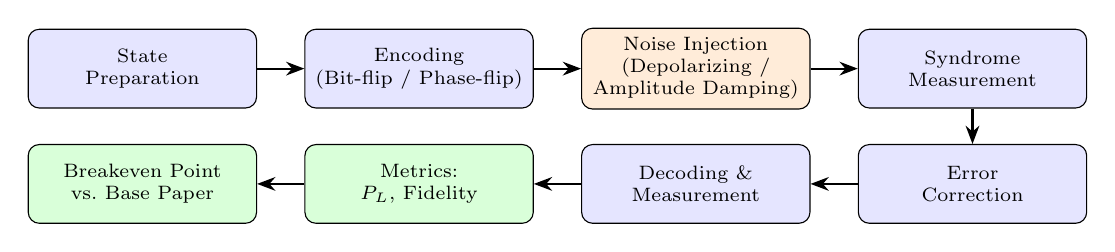
\begin{tikzpicture}[
    node distance=0.45cm and 0.6cm,
    box/.style={rectangle, draw, rounded corners, fill=blue!10, minimum width=2.9cm, minimum height=1cm, align=center, font=\scriptsize},
    noisebox/.style={rectangle, draw, rounded corners, fill=orange!15, minimum width=2.9cm, minimum height=1cm, align=center, font=\scriptsize},
    outbox/.style={rectangle, draw, rounded corners, fill=green!15, minimum width=2.9cm, minimum height=1cm, align=center, font=\scriptsize},
    arr/.style={-{Stealth}, thick}
]
\node[box] (state) {State\\Preparation};
\node[box, right=of state] (encode) {Encoding\\(Bit-flip / Phase-flip)};
\node[noisebox, right=of encode] (noise) {Noise Injection\\(Depolarizing /\\Amplitude Damping)};
\node[box, right=of noise] (syndrome) {Syndrome\\Measurement};
\node[box, below=of syndrome] (correct) {Error\\Correction};
\node[box, left=of correct] (decode) {Decoding \&\\Measurement};
\node[outbox, left=of decode] (metrics) {Metrics:\\$P_L$, Fidelity};
\node[outbox, left=of metrics] (breakeven) {Breakeven Point\\vs.\ Base Paper};
\draw[arr] (state) -- (encode);
\draw[arr] (encode) -- (noise);
\draw[arr] (noise) -- (syndrome);
\draw[arr] (syndrome) -- (correct);
\draw[arr] (correct) -- (decode);
\draw[arr] (decode) -- (metrics);
\draw[arr] (metrics) -- (breakeven);
\end{tikzpicture}
\end{frame}
% ---------------- Slide 10: Objectives ----------------
\begin{frame}{Objectives}
\begin{itemize}
    \item Implement a 3-qubit Bit-Flip Code and a 3-qubit Phase-Flip Code using Qiskit.
    \item Simulate Depolarizing and Amplitude Damping noise channels at probabilities from 1\% to 20\%.
    \item Measure and benchmark Physical Error Rates versus Logical Error Rates.
    \item Calculate the exact fidelity of the recovered quantum states post-correction.
    \item Identify the empirical pseudo-threshold / breakeven point, and compare it against the scaling law predicted by Thakur et al. (2025).
\end{itemize}
\end{frame}
% ---------------- Slide 11: Timeline ----------------
\begin{frame}{Timeline (12-Week Plan)}
\begin{itemize}
    \item \textbf{Weeks 1-2:} Literature review, Qiskit setup, theoretical validation.
    \item \textbf{Weeks 3-4:} Programming the 3-Qubit Bit-Flip and Phase-Flip circuits.
    \item \textbf{Weeks 5-6:} Mathematical modeling and injection of Depolarizing and Amplitude Damping noise (1\% to 20\%).
    \item \textbf{Weeks 7-8:} Execution of error detection and correction protocols.
    \item \textbf{Weeks 9-10:} Data collection (Physical/Logical Error Rates, Fidelity).
    \item \textbf{Weeks 11-12:} Benchmarking graphs, pseudo-threshold analysis, comparison with base paper, final documentation.
\end{itemize}
\end{frame}
% ---------------- Slide 12: Expected Outcomes ----------------
\begin{frame}{Expected Outcomes}
\begin{itemize}
    \item Working Qiskit implementation of 3-qubit bit-flip and phase-flip QEC circuits.
    \item Empirical physical-vs-logical error rate curves for two distinct noise channels.
    \item A measured pseudo-threshold / breakeven point for each noise channel.
    \item A direct comparison plot: base paper's predicted scaling curve vs.\ our measured data.
    \item Evidence for whether a minimal-overhead code follows the same theoretical trend claimed for large surface codes.
\end{itemize}
\end{frame}
% ---------------- Slide 13: References ----------------
\begin{frame}{References}
\footnotesize
\begin{enumerate}
    \item P. W. Shor, ``Scheme for reducing decoherence in quantum computer memory,'' \textit{Phys. Rev. A}, 1995.
    \item A. M. Steane, ``Error correcting codes in quantum theory,'' \textit{Phys. Rev. Lett.}, 1996.
    \item D. Gottesman, ``Stabilizer codes and quantum error correction,'' 1997.
    \item J. Chiaverini et al., ``Realization of quantum error correction,'' 2004.
    \item M. D. Reed et al., ``Realization of three-qubit QEC with superconducting circuits,'' 2012.
    \item A. D. C\'orcoles et al., ``Demonstration of a quantum error detection code,'' 2015.
    \item J. R. Wootton, ``Benchmarking near-term devices with quantum error correction,'' 2020.
    \item Google Quantum AI, ``Exponential suppression of bit or phase errors with cyclic error correction,'' \textit{Nature}, 2021.
    \item L. Postler et al., ``Demonstration of fault-tolerant universal quantum gate operations,'' 2022.
    \item A. Chatterjee \& S. Ghosh, ``Magic Mirror on the Wall: How to Benchmark QEC Codes Overall?,'' 2024.
    \item V. S. Thakur, A. Kumar, K. Dev, ``Quantum Error Correction in Green Communications: Toward Sustainable Quantum Networks,'' \textit{IEEE Trans. Green Commun. Netw.}, vol. 9, no. 4, pp. 1566--1576, Dec. 2025.
\end{enumerate}
\end{frame}
% ---------------- Slide 14: Thank You ----------------
\begin{frame}
\centering
\vspace{1.5cm}
{\Huge Thank You}
\vspace{0.5cm}
{\large Questions?}
\end{frame}
\end{document}
